% REMEMBER: You must not plagiarise anything in your report. Be extremely careful.

\documentclass{l4proj}

    
%
% put any additional packages here
%

\begin{document}

%==============================================================================
%% METADATA
\title{Espruino Tools - An asynchronous JavaScript library to control remote embedded devices [JavaScript, Promise, Arduino]}
\author{Callum McLuskey}
\date{24 March, 2023}

\maketitle

%==============================================================================
%% ABSTRACT
\begin{abstract}
    \textbf{THIS IS UNFINISHED}

    The personal usage of remote embedded devices is a growing area in engineering allowing for anybody to get started building robotics systems at home or even develop skill sets in programming and electronic engineering. A big name in this scene is Arduino a product which allows hobbyists to build and design systems to suit personal project needs; The Espruino project takes this in a different direction by utilising a JavaScript interpreter which aims to bring remote embedded systems programming to the web. This project intends to improve the development experience of remote embedded devices by refining the process and allowing users to focus more on their ideas and less on the semantics required to implement them. To achieve this the project introduces many packages providing functionality such as easy device connection[ADD LINK], peer-to-peer[ADD LINK] connection for mobile device inputs to be used, and the refined syntax to allow developers to get started regardless of skill or prior knowledge with wide and detailed documentation to avoid confusion when developing. In addition to this to further ease development, a CLI tool has been developed to create projects preset with all the functionality a beginner user could need, setting anybody up for programming Espruino devices, an activity which had no clear direction before of how to be done. By utilising user studies throughout the project a variety of users from different experience levels have been considered during the development process allowing for the project to be as accessible as possible.

\end{abstract}

\def\consentname {Callum McLuskey} % your full name
\def\consentdate {23 March 2023} % the date you agree

\educationalconsent

\tableofcontents

%==============================================================================
%% Notes on formatting
%==============================================================================
% The first page, abstract and table of contents are numbered using Roman numerals and are not
% included in the page count. 
%
% From now on pages are numbered
% using Arabic numerals. Therefore, immediately after the first call to \chapter we need the call
% \pagenumbering{arabic} and this should be called once only in the document. 
%
% Do not alter the bibliography style.
%
% The first Chapter should then be on page 1. You are allowed 40 pages for a 40 credit project and 30 pages for a 
% 20 credit report. This includes everything numbered in Arabic numerals (excluding front matter) up
% to but excluding the appendices and bibliography.
%
% You must not alter text size (it is currently 10pt) or alter margins or spacing.
%
%
%==================================================================================================================================
%
% IMPORTANT
% The chapter headings here are **suggestions**. You don't have to follow this model if
% it doesn't fit your project. Every project should have an introduction and conclusion,
% however. 
%
%==================================================================================================================================
\chapter{Introduction}

% reset page numbering. Don't remove this!
\pagenumbering{arabic} 


\section{Motivation}

\text 
The area of remote embedded systems has seen significant growth in recent years due to the growing need for interconnected devices and the Internet of Things (IoT). It offers developers the chance to craft physical objects that interact with the real world, resulting in a final product they can take pride in. However, the current setup of remote embedded systems, like Arduino, has a challenging learning curve due to the utilization of C++ as the programming language.
\\ \\
An alternate solution to this is presented by Espruino devices, which make use of JavaScript, a language that is more accessible to a broader range of developers. Espruino presents a reduced entry barrier and eliminates the requirement to learn a new language, which can be daunting for some. This makes it easier for developers to commence with remote embedded systems and begin constructing their projects.
\\ \\
Even though using Espruino devices can tackle some of the issues linked to traditional remote embedded systems, it still gives a restricted comprehension of JavaScript and its fundamental technologies. This can result in a limited skill set that is not readily transferable to other areas of software engineering.
\\ \\
This project aims to tackle these challenges by providing developers with a cutting-edge JavaScript-based platform for building their remote embedded systems. By utilizing contemporary JavaScript, developers will gain a deeper understanding of the language and its features, as well as acquire in-demand skills that can be applied to other areas of software engineering.
\\ \\
This project aims to help prepare future programmers and software engineers for work within the embedded systems allowing them to achieve working systems as well as allowing for the development of in-demand skills through the usage of modern JavaScript with easy access to work with any modern JavaScript of their choice.

\section{Aims / Goals}

\textbf{[THIS IS A PLACEHOLDER NEEDS EXPANDING]}

\text This effort will create a collection of packages aimed at lowering the threshold for individuals looking to get into programming in the remote embedded systems area, yet still offering benefits for experienced coders through its streamlining of the current Espruino implementation. Additionally, these modules are constructed with a strong emphasis on web technologies, providing both novice and seasoned developers with an opportunity to deepen their understanding of current web technologies while working on their embedded systems.



%==================================================================================================================================
\chapter{Background}

\textbf{NONE OF THIS IS FINAL AND NEEDS TO BE REWRITTEN}

\section{Something about current state of learning programming}

\section{Espruino Devices}
\text 
The Espruino micro-controller provides an innovative solution for individuals seeking to materialise their electronics project aspirations. With a JavaScript interpreter and in-built amenities such as WiFi and Bluetooth, this device makes it effortless for individuals of diverse programming proficiency to dive in. The Espruino ecosystem caters to hobbyists and students eager to learn about electronics and programming. These micro-controllers can be blended seamlessly with other hardware and software systems, opening up a world of possibilities for electronics projects.

    
\subsection{UART}
\text Espruino devices communicate with the browser by utilising UART, or Universal Asynchronous Receiver/Transmitter, a widely used communication protocol in the world of micro-controllers and embedded systems. It doesn't require a fixed clock rate between the sender and receiver and instead uses start and stop bits for data transmission synchronization. \textbf{[EXPAND ON THIS AND INCLUDE MORE ABOUT HOW IT ACTUALLY WORKS]}


\begin{center}
    % ADD FIGURE DETAILS LIKE A CAPTION
    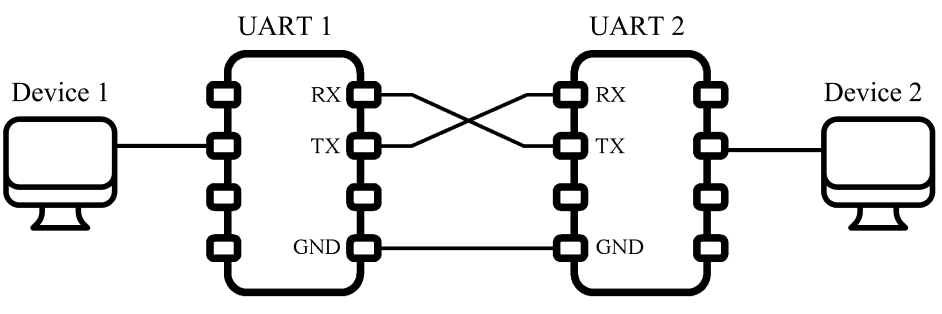
\includegraphics[width=60mm,scale=0.5]{dissertation/images/UART_diagram.png}
\end{center}




\subsection{WebBluetooth}
\text UART connection with a web browser as mentioned above is facilitated via WebBluetooth. WebBluetooth is an aspect of the Web API that facilitates communication between web applications and Bluetooth Low Energy (BLE) devices. This technology allows web developers to control and access BLE devices using JavaScript, providing a streamlined and standardized approach.

WebBluetooth represents a milestone in the integration of BLE devices into the web, as it offers a common platform for web developers to interact with these devices, regardless of their origin or operating system. It expands the possibilities for BLE devices, including the ability to control smart home technology or track fitness information through a web application.

\section{Package Development}

Passage about modern package development

\subsection{NPM}
\text NPM is a tool utilized in the world of JavaScript programming to manage software packages. It serves as a centralized hub for individuals to quickly find, install, and handle an extensive collection of libraries and packages for their projects. NPM empowers developers to share their packages and work together on open-source initiatives. Due to its large repository of packages, NPM has become a must-have tool for contemporary JavaScript development.

\subsection{NPX}
\text NPX is a tool for executing Node.js packages, including those installed through npm (Node Package Manager). It allows users to run a package's binary without having to install it globally on their system. This is useful for testing packages or trying out new features without affecting other parts of the system. NPX also enables developers to run packages with specific versions, rather than relying on the globally installed version. It provides a convenient and efficient way to run packages, making it a popular tool in the Node.js ecosystem.

\section{Device to device communication}

Small paragraph surrounding the current state of communicating between different devices. potentially mention adoption 

\subsection{WebRTC}
\text WebRTC (Web Real-Time Communication) is a freely available resource that enables web browsers and devices to communicate voice, video and data in real-time without the need for additional software. This technology has been engineered to operate on a variety of networks and platforms, resulting in low lag and excellent audio and video streaming quality for web-based communication. Popular uses for WebRTC include video conferencing, live streaming, online gaming, and file sharing.

\section{Open Source}
\text Open source pertains to a licensing model for software that enables the public to view and modify the source code. It is developed and maintained by a community of contributors, rather than by a single entity. The objective of open source is to promote collaboration, transparency, and innovation in software development, and to give users more control and choice over their software. Notable open source projects include the Linux operating system and the Python programming language.

\section{Existing Projects}
\text Espruino native language / online IDE.

%==================================================================================================================================
\chapter{Analysis/Requirements}
\section{Functional Requirements}
\subsection{Must Have}
\text An overhaul to the UART.js package incorporating modern ECMAScript standards, A package which simplifies the development process to allow focus on learning or building, demos to display how this package helps, A well populated documentation site (helps new and existing programmers, fixes issue with standard espruino having hard to navigate documentation)
\subsection{Should Have}
\text Speed improvements over original UART.js.
\subsection{Could Have}
\text placeholder text
\section{Non-Functional Requirements}
\text What are non-functional requirements
\subsection{Must Have}
\text A simplified entry point for new programmers, Ability to showcase projects through easy hosting (i.e. github pages)
\subsection{Should Have}
\text placeholder text
\subsection{Could Have}
\text placeholder text

\section{Specification changes}
\subsection{Peer to Peer}
\text A separate package which allows users to easily integrate a connection between mobile devices and their browser to bridge the gap in espruino only being able to be used on specific devices.

\subsection{Transpiler}
\text Provide a program which can translate ... to fully allow for the code to work on any given espruino platform be that their online IDE or even directly written onto the device. Mention this came up after discussion about providing an online environment and ability for less boxed in code processing.

\subsection{NPX Tool}
\text Improve the time required to set up a development environment to allow more focus on the code and less on the logistics of how to get an environment set up.

\subsection{Online Environment}
\text Allow users to have an environment in which they can test new features without setting up a whole development environment. This can be used to test functionality or even develop whole projects.
%==================================================================================================================================
\chapter{Design}
How is this problem to be approached, without reference to specific implementation details? 
\section{Organisations}
\subsection{Github}
\text something about open source, keeping everything together.
\subsection{NPM}
\text scoped packages, keeps everything together.
\section{NPX Tool Repositories}
\text why react, vue, typescript. Why have `--clean-install`, `--peer`
\subsection{Git Submodules}
\text Why.
\subsection{Tags}
\text `--clean-install` `--template` `--peer`
\section{UI/UX Improvements}
\text modals, prototyping (Figma)
\section{Agile Methodologies}
\text choice for software architecture.
%==================================================================================================================================
\chapter{Tools / Technologies}

The section will discuss the usage of technologies throughout the project splitting them into relevant sections containing technologies used by specific areas of the project.

\section{general}

The packages discussed below are used throughout the full ecosystem and help provide the vital structure of the package development.

\subsection{Typescript}
\text Typescript offers several benefits over JavaScript when building a software package. It is a statically typed super-set of JavaScript, providing improved code quality through static typing and a better understanding of large code-bases through its type system. Typescript also offers better scalability with features like interfaces, classes, and modules, as well as better tooling support through better integration with modern development tools. Additionally, Typescript includes features that are part of upcoming versions of JavaScript, making code written in it future-proof.

\subsection{NPM}
\text Using the Node Package Management (NPM) system when developing a JavaScript application presents numerous benefits. NPM eases the management of packages, guaranteeing the right version is installed correctly. The NPM network boasts a significant community of developers and a vast collection of programs, minimizing the need for repeated efforts and making it easy to integrate new features. NPM standardizes the system for versioning packages and enables seamless distribution of programs to the community. The adoption of NPM also enables automation of processes like building, testing, and deploying packages, reducing the workload associated with managing the project.


\subsection{UNPKG}
\text The utilization of inline JavaScript imports through UNPKG provides numerous advantages. The ability to integrate small amounts of code through inline imports enables a fast and straightforward method for experimenting with various components and evaluating different solutions. Utilising both inline imports and NPM package imports simultaneously presents a versatile and efficient development process, empowering developers to select the most suitable approach for their project needs.

\subsection{Azure DevOps}
\text Azure DevOps is a unified platform for software development that consolidates various tools and services. It offers a complete solution for source control, continuous integration/testing/deployment, and project management. Azure DevOps streamlines the development process by providing features such as automated builds, continuous deployment, and team collaboration, outperforming alternative approaches that utilize individual tools like Jenkins or Jira.

\subsection{Webpack [!!NEEDS WORK!!]}
\text can use new javascript features and compile into older widely used, enables typescript.Other webpack benefits converts all code into es5 by choice (why es5)
Why not parcel or snowpack or another bundler

\subsection{React [!!NEEDS WORK!!]}
\text Why is react used for demos and online IDE vs Vue, Angular, vanilla or any other. Using a framework benefits.
comparing frameworks

\subsection{Husky [!!NEEDS WORK!!]}
\text what is it (runs git hooks), what are git hooks
auto package versioning
commit sanitizing

\section{CLI tool [!!NEEDS WORK!!]}

The CLI tool takes a different approach in development to the NPM packages as there is a requirement to be run through the command line.

\subsection{NPX [!!NEEDS WORK!!]}
\text NPX is a command line package runner allowing for the execution of node based JavaScript packages through a specified command. This has avid usage within the javascript development scene for building starting point directories, popular examples include React's create-react-app and Vue's vue-cli to name a few.

\section{Peer [!!NEEDS WORK!!]}

Integrating a peer-to-peer connection without utilising a self built and hosted back-end system provided an issue.

\subsection{peerJS}
\text PeerJS provides an all-in-one solution which utilises WebRTC removing the issue of building a home made WebSocket back-end system to allow for real-time communication between devices this approach allows for developers to keep the simplicity of hosting static files without having to worry about the maintenance and cost of hosting of a back-end system.

\subsection{qrcode Package [!!NEEDS WORK!!]}
\text - ease of use

\section{Documentation [!!NEEDS WORK!!]}

\subsection{Docusaurus [!!NEEDS WORK!!]}
\text why this over jekyll, hugo. MDX, agolia search

\section{Transpiler [!!NEEDS WORK!!]}

\subsection{Esprima [!!NEEDS WORK!!]}
\text why use existing parse/tokeniser, Mozilla standard for Javascript. Avoid re-inventing the wheel.
\subsection{EsCodeGen [!!NEEDS WORK!!]}
\text Why use this instead of building your own, Mozilla standard for Javascript. Avoid re-inventing the wheel.
%==================================================================================================================================
\chapter{Implementation}
What did you do to implement this idea, and what technical achievements did you make?
\section{Feature / Packages / Web Apps}
You can't talk about everything. Cover the high level first, then cover important, relevant or impressive details.
\subsection{core}
\subsection{peer}
\subsection{uart}
\subsection{create-espruino-app}
\subsection{online IDE}
\subsection{Transpiler}

\section{Documentation}
\text Just why this is so important for a collection of packages.
\section{CI/CD}
\text How the product functionality was checked, Azure using the pipeline to run build checks and tests.

\section{Testing}
\text JEST, javascript testing suite. Cypress,Front end testing suite (this may only be applicable for demo site and online IDE.


\section{Deployment}
\subsection{Packages}
\text How the packages are deployed using azure pipelines ,npm and unpkg to host package.
\subsection{Web Apps}
\text How the web apps are deployed. Vercel, what is vercel and why use it?



\chapter{Evaluation} 
How good is your solution? How well did you solve the general problem, and what evidence do you have to support that?

\section{User Feedback}
\section{Core}
\subsection{Speed Comparison}
\section{Peer}
\subsection{Speed Comparison}
\section{Transpiler}

%==================================================================================================================================
\chapter{Conclusion}    
Summarise the whole project for a lazy reader who didn't read the rest (e.g. a prize-awarding committee).
\section{Summary}
\section{Reflection}
\section{Future Work}
\section{Limitation}

%==================================================================================================================================
%
% 
%==================================================================================================================================
%  APPENDICES  

\begin{appendices}
\chapter{Appendices}
\end{appendices}

%==================================================================================================================================
%   BIBLIOGRAPHY   

% The bibliography style is abbrvnat
% The bibliography always appears last, after the appendices.

\bibliographystyle{abbrvnat}

\bibliography{l4proj}

\end{document}
